\documentclass[12ptr]{article}
\usepackage[a4paper,width=150mm,headheight=110pt,top=25mm,bottom=25mm]{geometry}
\usepackage[utf8]{inputenc}
\usepackage{listings}
\usepackage{graphicx}
\usepackage{pgffor} 
\usepackage{float}
\usepackage{graphics} 
\usepackage{fancyhdr}
\usepackage{titling}
\usepackage{hyperref}
\usepackage{caption}
\usepackage{subfig}
\usepackage{amsmath}

%\renewcommand\maketitlehooka{\null\mbox{}\vfill}
%\renewcommand\maketitlehookd{\vfill\null}


%----------------------------------------------------------------------------------------
%	Title Page
%---------------------------------------------------------------------------------------
\begin{document}

\vspace*{5cm}
 \begin{center}
{\huge \bf GPU Computing for Bionanotechnology}\\[0.2cm]
{\large \bf Mentor: Prof. Aleksei Aksimentiev}\\[0.2cm]
{\large Mentee: Swan Htun (SPIN)}\\[0.2cm]
{July 23 2019}\\[0.5cm]
\end{center}

\begin{figure}[!ht]
    \centering
    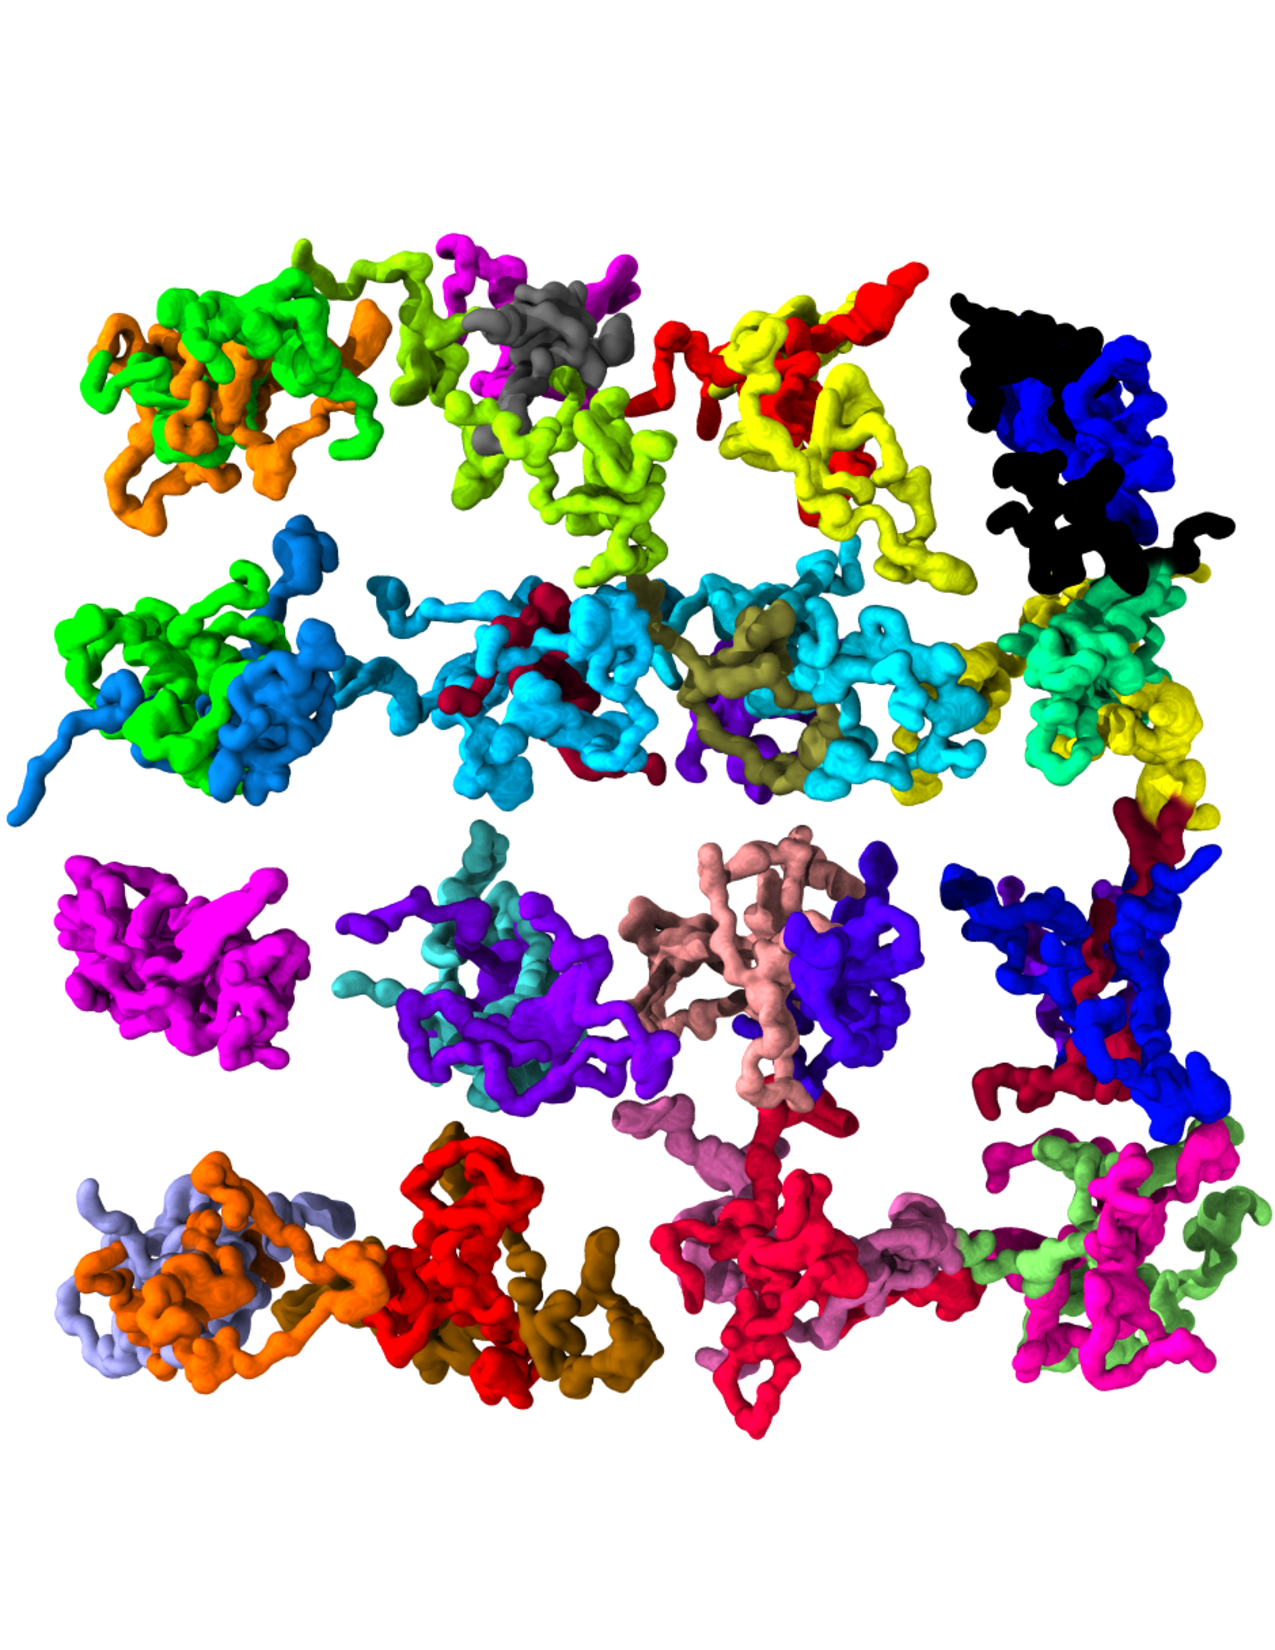
\includegraphics[width=6cm]{fus400_64_first.pdf}
    \qquad
    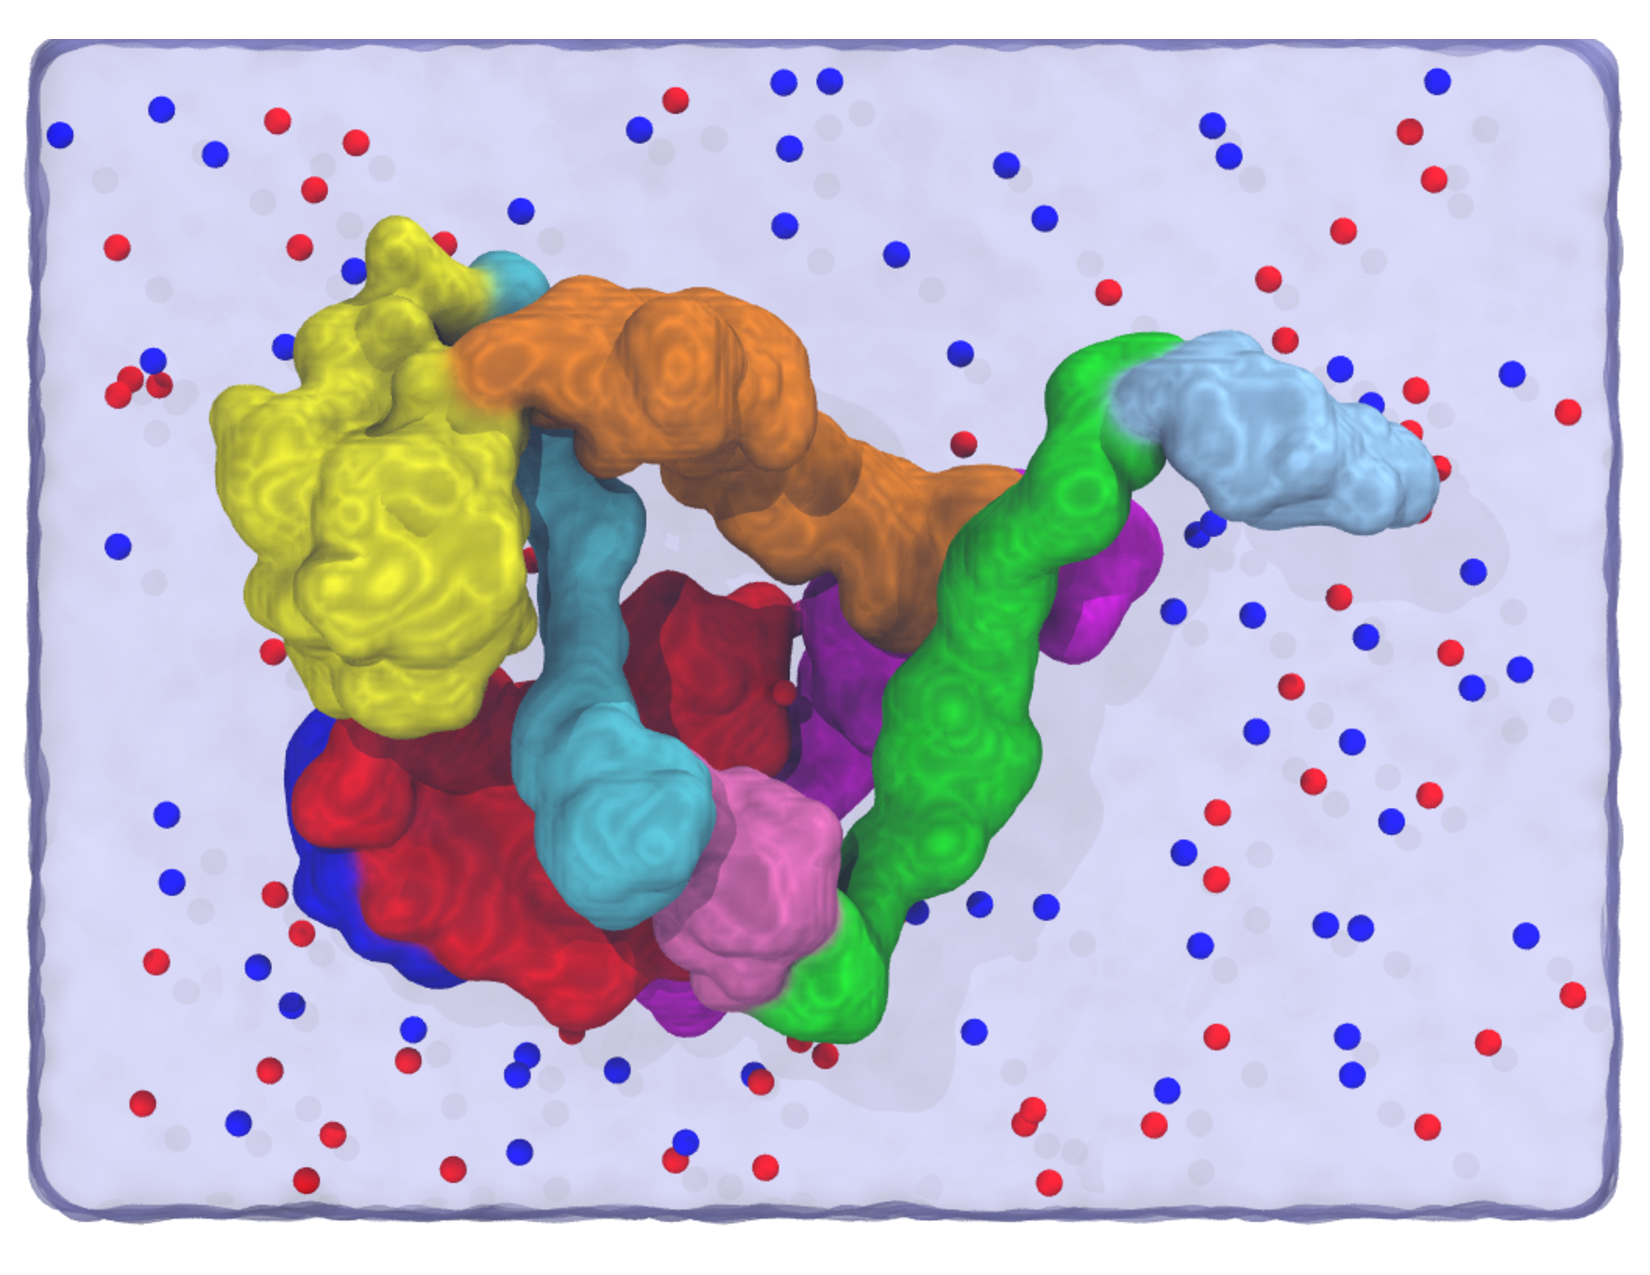
\includegraphics[width=7cm]{all_atom_fus1.pdf} 
\end{figure}


\newpage


%----------------------------------------------------------------------------------------
%	Table of Contents
%---------------------------------------------------------------------------------------
%\addtocontents{toc}{\setcounter{tocdepth}{1}} % Set depth to 1
\tableofcontents
\newpage

\section{Abstract}
Biomolecular condensates are membraneless organelles found in Eukaryotic cells that are formed by liquid-liquid phase separation (LLPS) and display liquid-like properties \cite{Patel_15}. An important constituent of certain condensates is the Fused in Sarcoma (FUS) protein, which is an RNA-binding protein involved in various cellular processes such as DNA repair, RNA transport and damage response \cite{Patel_15}. The FUS protein is essential for the condensate to undergo the LLPS process in vivo and the FUS protein itself undergoes LLPS in vitro \cite{Ali_18}. Our current goal is to computationally investigate phase separation in the FUS protein by studying the phase separation process of both wild-type (WT) and mutant FUS protein under various  temperatures and concentrations. In this paper, we present the results of the Brownian Dynamic simulations run at various temperatures ranging from $295$K to $450$K. The results suggest that the cutoff temperature for phase separation is around $415$K. Further simulations at different concentrations are being carried out to quantify the effects of concentration in phase separation process as well as how certain mutations interfere with phase transitions of FUS. 

\section{Introduction}

Biological cells have compartmentalized cellular space for efficient regulation of biochemical reac-tions by isolating certain biochemical process from the rest of the cell by bounding the reactions inside membraneous organelles. Eukaryotic cells, however, also have many organelles that lack membrane-enclosed structures \cite{Mullard_19}, such as stress granules, and nucleoli \cite{Mullard_19}. Such membraneless organelles are commonly known as biomolecular condensates \cite{Banani_17}. Due to their highly dynamic nature, they have liquid-like properties and are formed via liquid-liquid phase separation (LLPS) process as a response to specific biochemical signals \cite{Banani_17}. Such properties include the rapid exchange of their constituent molecules with the surrounding cytoplasm or nucleoplasm \cite{Mullard_19} as well as the ability to deform and freely flow around surfaces of other intracellular structures while under shear stress \cite{Banani_17}. They also undergo fusion and fission \cite{Patel_15, Mullard_19, Banani_17}.\\[0.01cm]

These condensates have specific macromolecular composition that can be classified qualitatively into two types: clients, which are preferentially recruited as part of the condensate, and scaffolds, which are required for the formation of the condensate. The majority of the condensate is comprised of clients \cite{Banani_17}.\\[0.01cm]

The properties and molecular mechanism of these biological condensates have become an interesting topic of research, specifically intrinsically disordered proteins like FUS, as growing evidence suggests their implication in pathogenesis of amyotrophic lateral sclerosis (ALS) and frontotemporal dementia (FTD) \cite{Deng_14}. The physical process involved in biomolecular condensate formation (i.e, phase separation) and certain biomolecules involved are both known, but the precise physical and molecular mechanism of formation and its related processes are still unknown. Thus, it’s still a challenge to relate specific features and properties of the condensates with the corresponding biological function, which is essential to understanding how aberrations in them contribute to disease. \\[0.01cm]

\subsection{Fused in Sarcoma (FUS)}

Each individual FUS protein is made up of 526 amino acids and consists of both ordered and disordered regions that can be divided into a prion-like domain and the RNA binding domain \cite{Murray_17}. The phase separation process has been experimentally determined to be driven primarily by the interactions between tyrosine residues from prion-like domains (PLDs) and arginine residues from RNA-binding domains (RBDs) \cite{Wang_18}. The PLDs consist mainly of intrinsically disordered regions (IDRs) that are low in amino acid diversity (polar residues and aromatic residues) \cite{Wang_18}. Such domains are highly prone to aggregation and have been associated with pathogenesis of diseases such as ALS. Mutations in PLDs have been found to accelerate the conversion of the liquid-like droplets of FUS to solid-state, which is detrimental \cite{Patel_15}.

\newpage

\section{Methodology}
Aspects of phase separation process are simulated using all-atom Molecular Dynamics (MD) and Atomic Resolution Brownian Dynamics (ARBD) simulations. The molecular events involved in phase separation occur at a time scale too fast to resolve experimentally, which is one of the advantages of using computational methods to investigate LLPS. MD numerically solves Newton’s equations of motion for each atom in the system to determine the position at each time step and therefore provides atomic-level resolution. ARBD uses Langevin equations of motion to obtain the trajectory of the atoms and does not provide atomic-level resolution since the system must be coarse-grained. The raw output data from both simulations gives the trajectory of all atoms (or coarse-grained particles) of the system. The trajectory is then analyzed to gain insight into the phase separation process. VMD is used to visually aid in the study of LLPS process of FUS. 

\subsection{Software \& Applications Used}
ARBD is a GPU-enabled code that takes advantage of the processing power of the GPUs to facilitate fast simulations and achieves better computational efficiency for large systems in compa-rison to all-atom MD simulations. Python script is used to interact with ARBD. Since the simulation of phase separation phenomena happens at a long time scale, we mainly utilize the BD simulations.
Visualizations and the all-atom model of FUS are built using the VMD software.
All-atom MD simulations are run using NAMD software on Stampede2 supercomputer.\\

We began by building a complete all-atom model of FUS protein using publicly available data of the atomic coordinates and the structural information of each ordered segment of FUS protein on Protein Data Bank: \href {http://www.rcsb.org}{http://www.rcsb.org}. As no structures are available for the disordered regions, their structures are generated from the amino acid sequence using the Avogadro software. Then, each individual segments are linked using VMD. From the all-atom model, we build the CG model of FUS as seen in Fig. \ref{fig:fus_both} using the python. 

\begin{figure}[!ht]
\centering
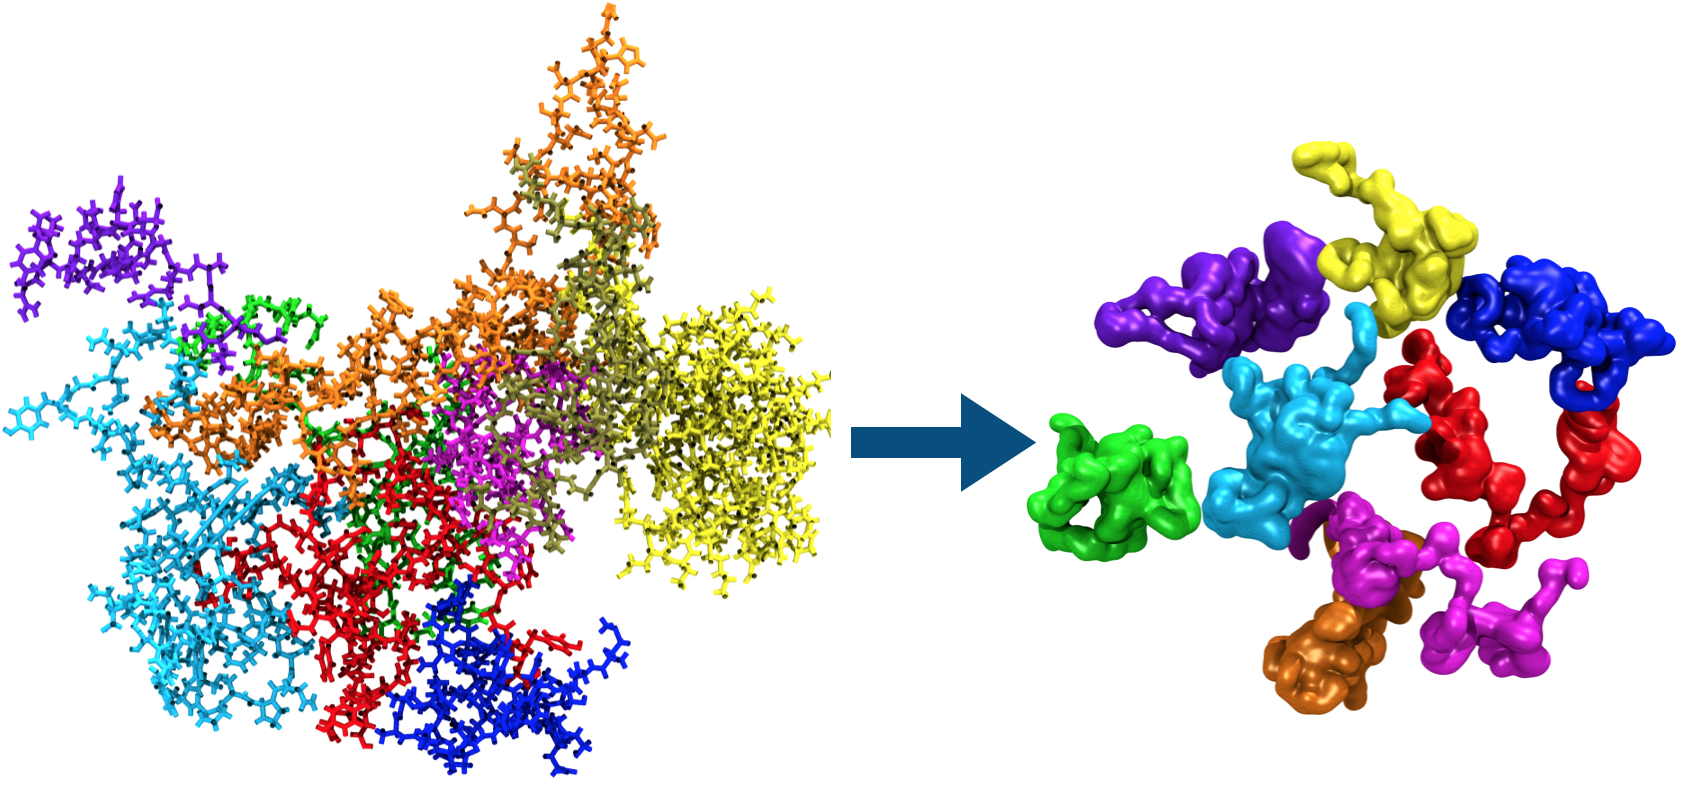
\includegraphics[width=6in]{together_b}
 \caption {\small All-atom model represented in `bonds' presentation (left) and coarse-grain model represented using `quicksurf' (right) of FUS  using VMD. As shown, there are 1 protein in all-atom system and 8 proteins in the CG sytem.}
 \label{fig:fus_both}
\end{figure}


\subsection{Simulation conditions}
All-atom simulations of WT FUS protein are run at $300$K with NPT conditions. The ARBD simulations of 8 WT FUS proteins are run at $295$K, $350$K, $400$K, $410$K, $420$K, $430$K, $440$K and $450$K in NVT conditions for over 10 $\mu s$. Another set of ARBD simulations of 64 WT FUS proteins as well as the mutant FUS proteins at similar temperatures are also being run to reveal the impact of concentration and mutations on phase separation. We also ran all-atom simulation of FUS protein for 100$ns$. It's important to know the concentration  $[FUS]$ of FUS in the system, which can be calculated via

\[ [FUS]=\frac{n}{N_A} \cdot \frac{1}{V} \]

\noindent where $n$ is the number of FUS proteins, $N_A$ is Avogadro's number, and $V$ is the volume of simulation box. 



\section{Results}

When looking at the simulated trajectory of the FUS protein over 8 $\mu s$ using VMD, we can see that at temperatures lower than $415$K, proteins coalesce to form a cluster or a few clusters as seen in Fig. \ref{fig:fus_350} (b). We created density maps of the protein densities to see the density distribution of the system Fig.\ref{fig:density}. We should expect the more homogeneous system, the one that did not coalesce to have a more uniform density map. Then, FFT is applied to the density map to quantify the phase transition from homogeneous to inhomogeneous phase, Fig \ref{fig:fft}(b). The normalized density fluctuations are analyzed to observe the temperature at which phase separation occurs. 

\begin{figure}[!ht]
    \centering
    \subfloat[The state of FUS proteins at the start of simulation.]{{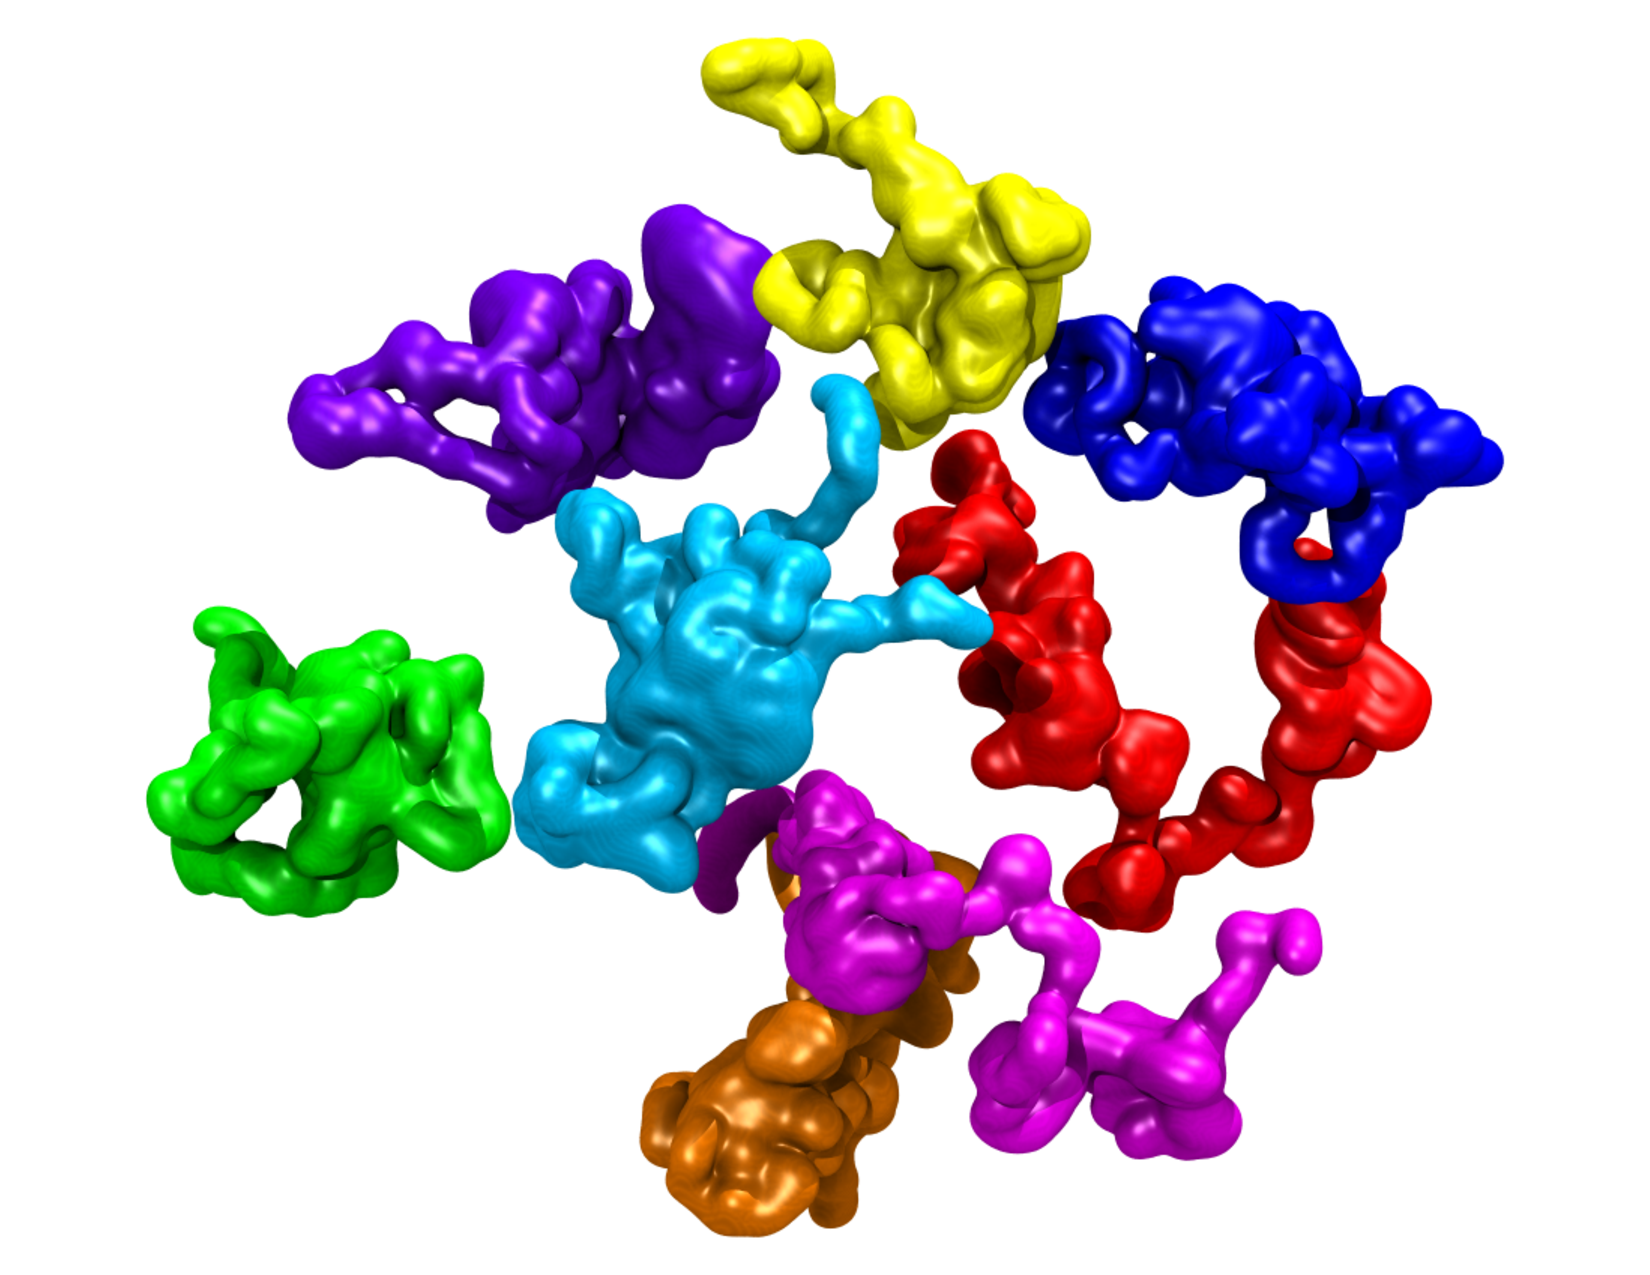
\includegraphics[width=6cm]{fus350_first.pdf} }}
    \qquad
    \subfloat[The state of FUS proteins at the end of 10 $\mu s$ simulation.]{{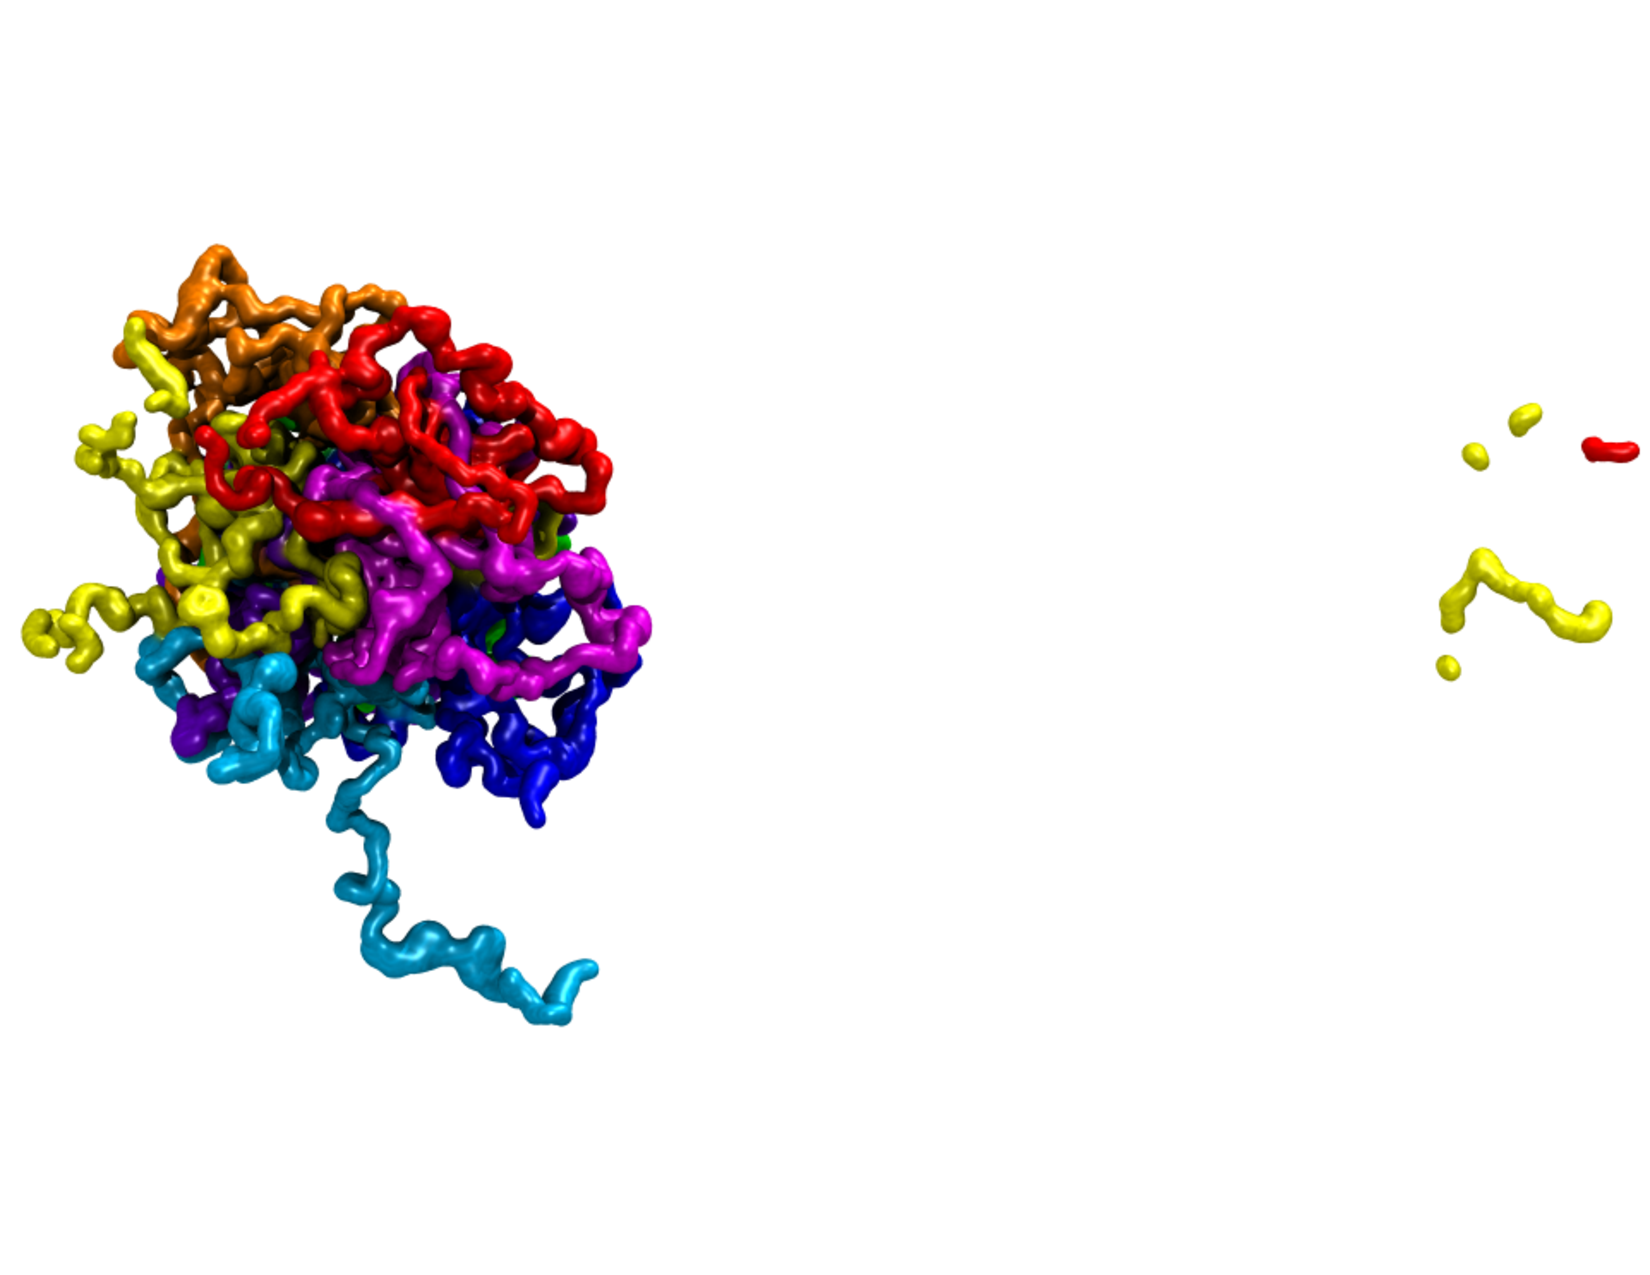
\includegraphics[width=8cm]{fus350_8_last.pdf} }}
    \caption {\small ARBD Simulation of FUS proteins. 8 FUS proteins were run at $350$K in a 825 $\mathring{A}^{3}$ resulting in 23.65 $\mu M$. The total number of atoms present were 43444.}
    \label{fig:fus_350}
\end{figure}

\begin{figure}[!ht]
    \centering
    \subfloat[The state of FUS proteins at the start of simulation]{{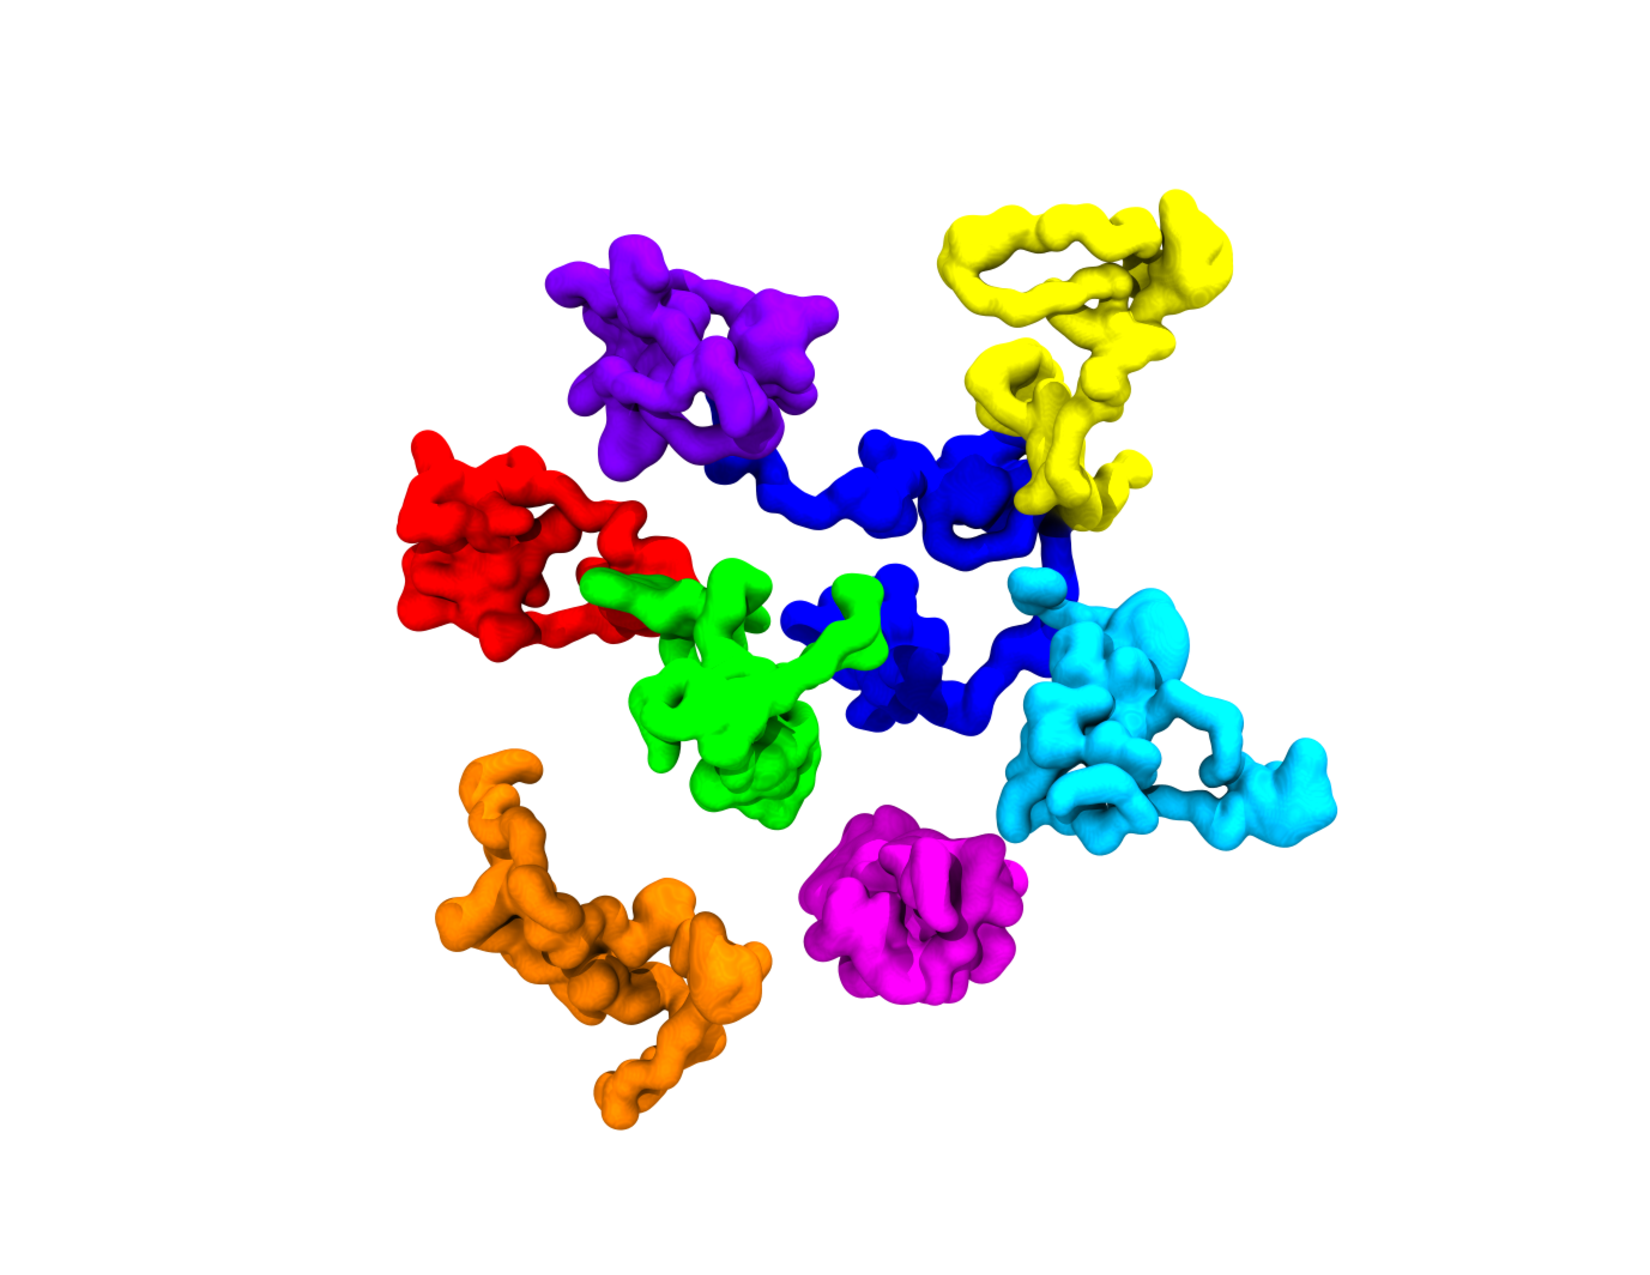
\includegraphics[width=6cm]{fus450_first.pdf} }}
    \qquad
    \subfloat[The state of FUS proteins at the end of 10 $\mu s$ simulation]{{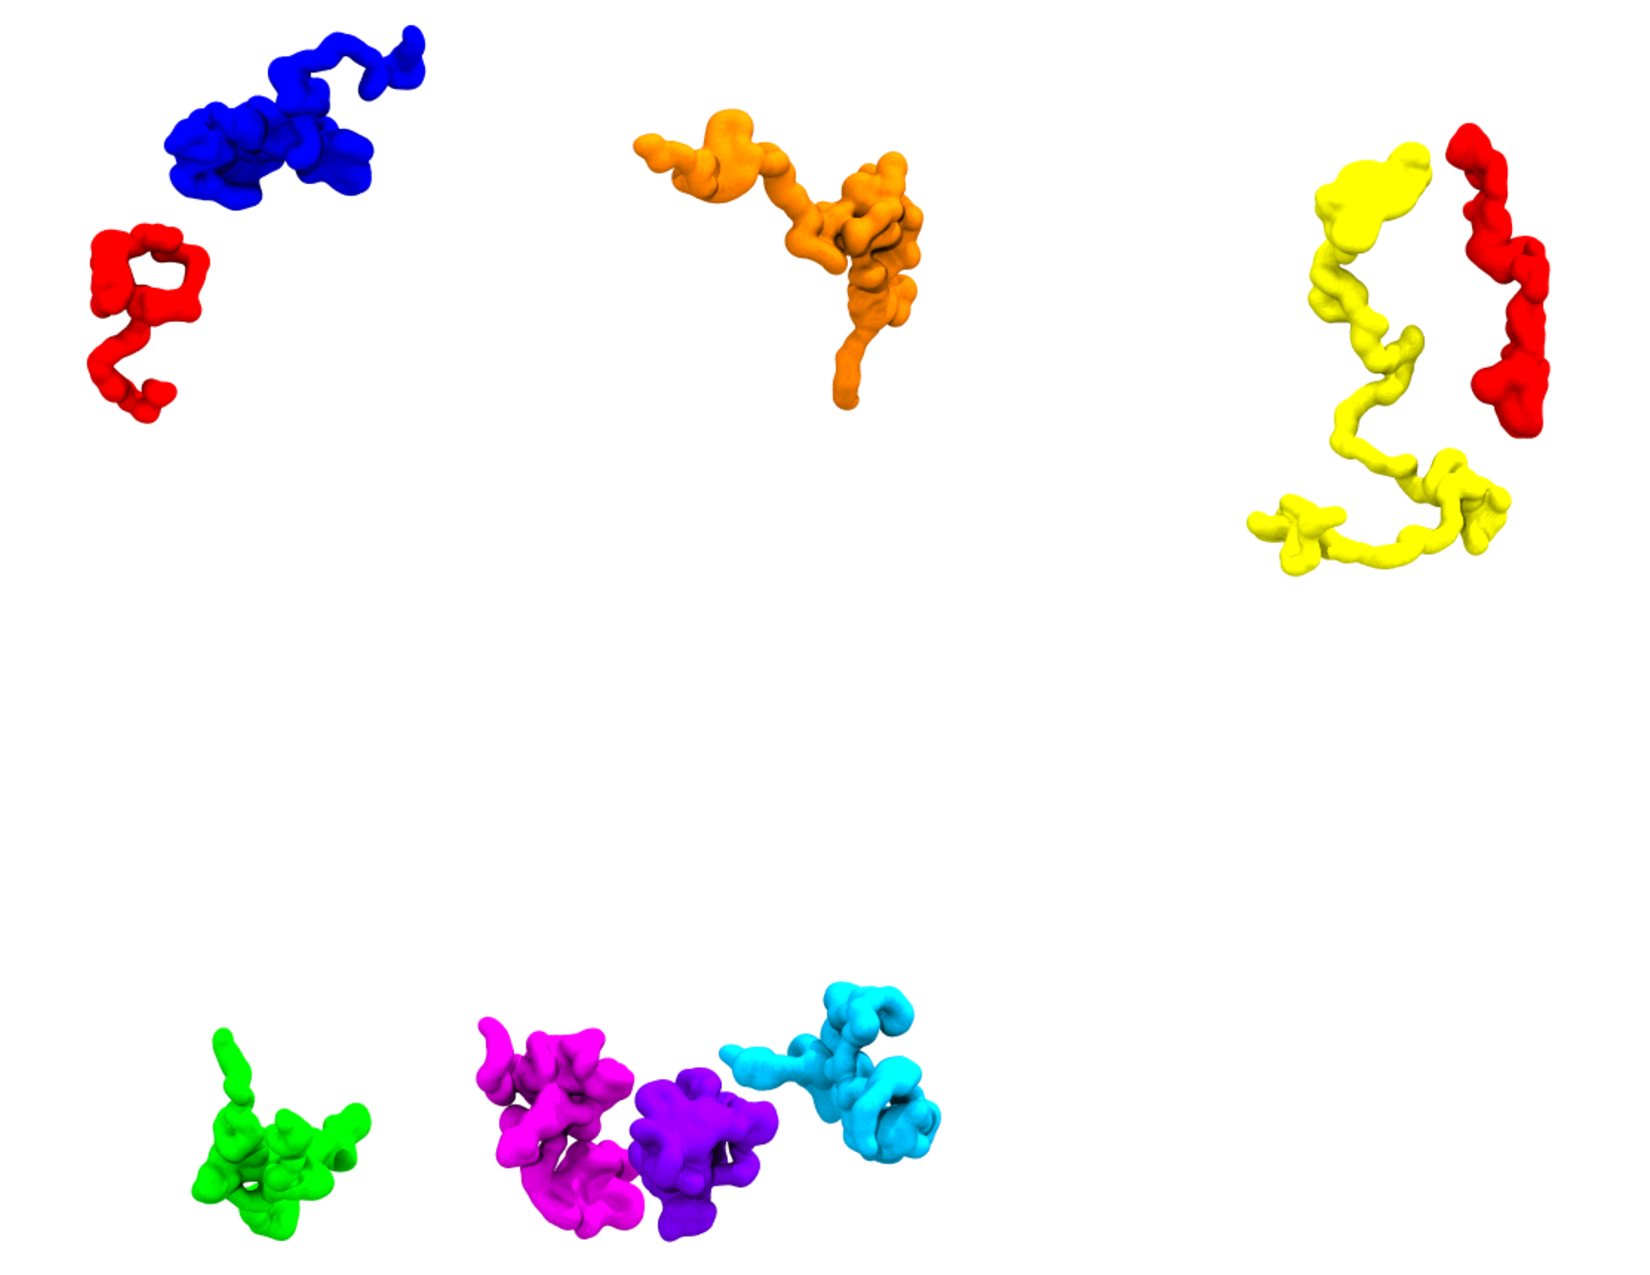
\includegraphics[width=8cm]{fus440_end.pdf} }}
    \caption {\small ARBD Simulation of FUS proteins. 8 FUS proteins were run at $450$K in a  825 $\mathring{A}^{3}$ resulting in 23.65 $\mu M$. The total number of atoms present were 43444.}
    \label{fig:fus_430}
\end{figure}

\begin{figure}[!ht]
    \centering
    \subfloat[$350$K ]{{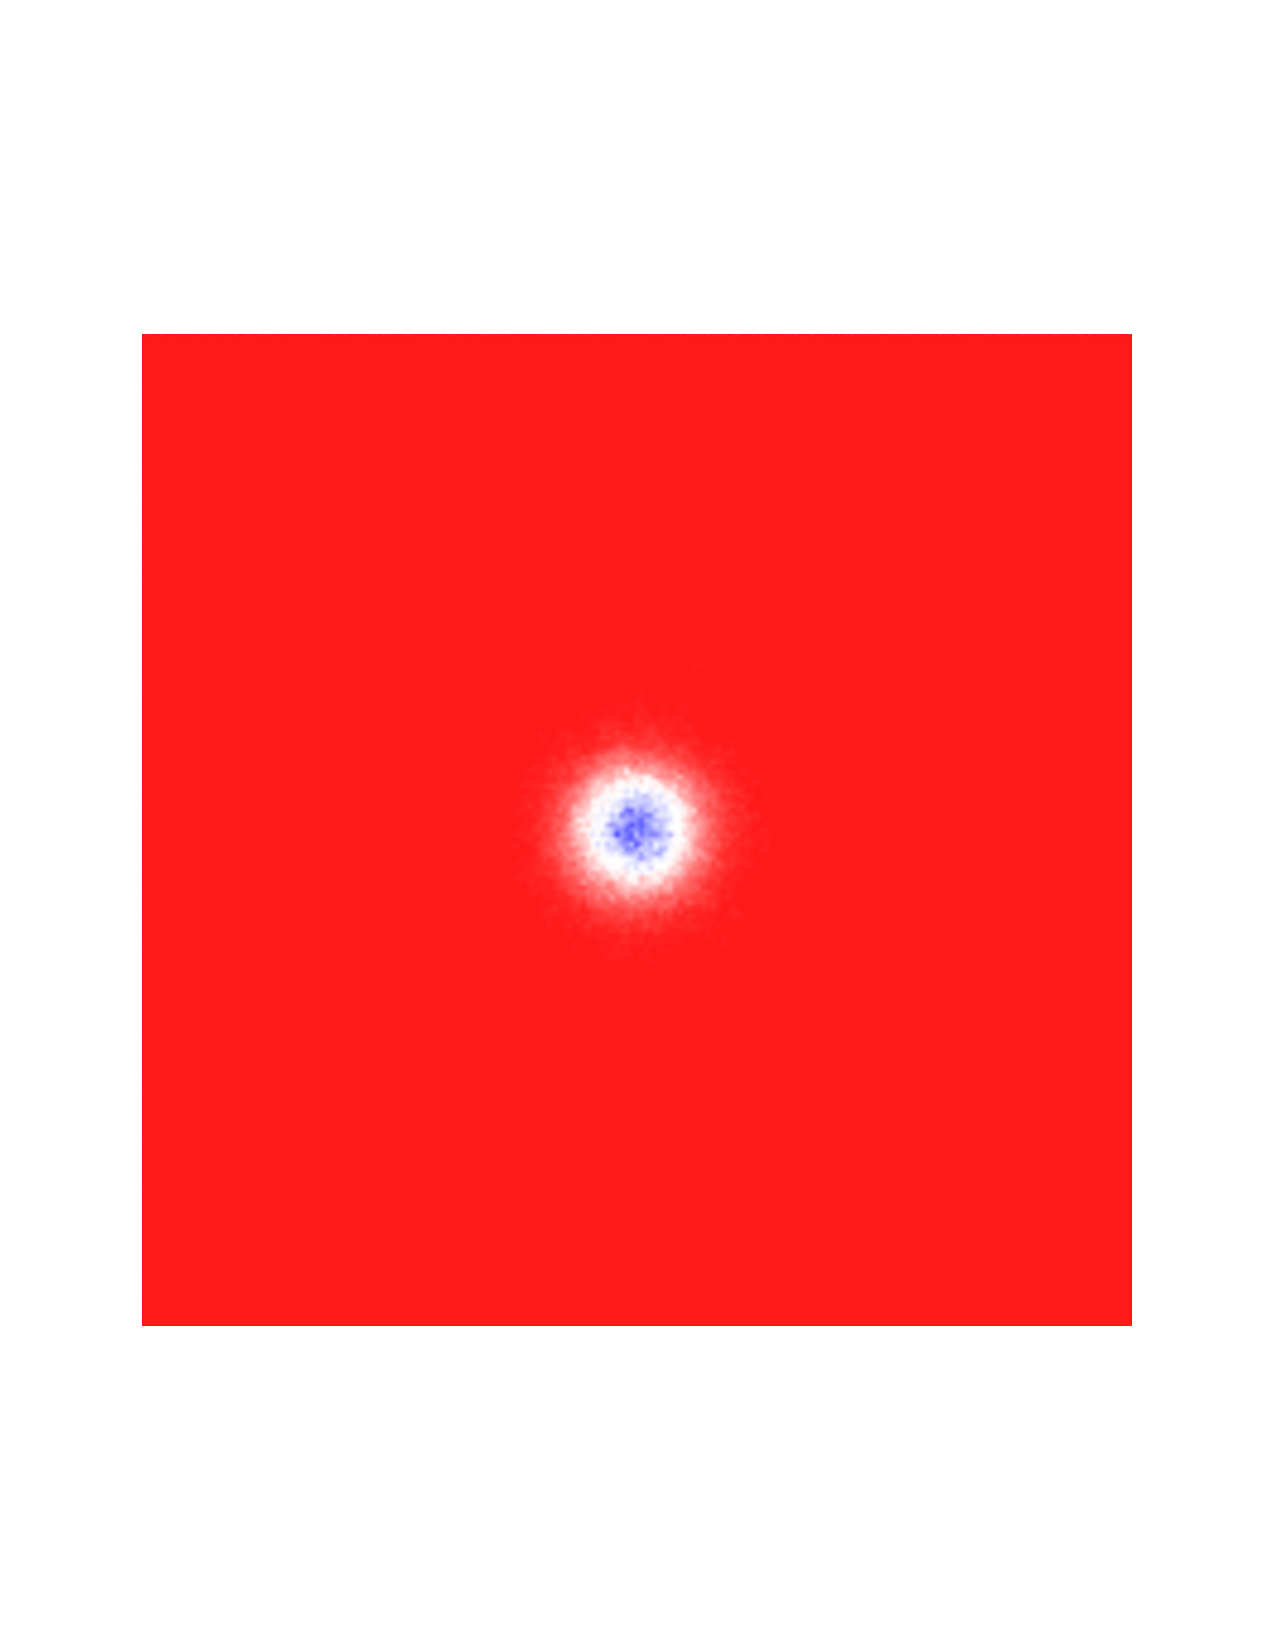
\includegraphics[width=7cm]{fus350_density.pdf} }}
    \qquad
    \subfloat[$450$K]{{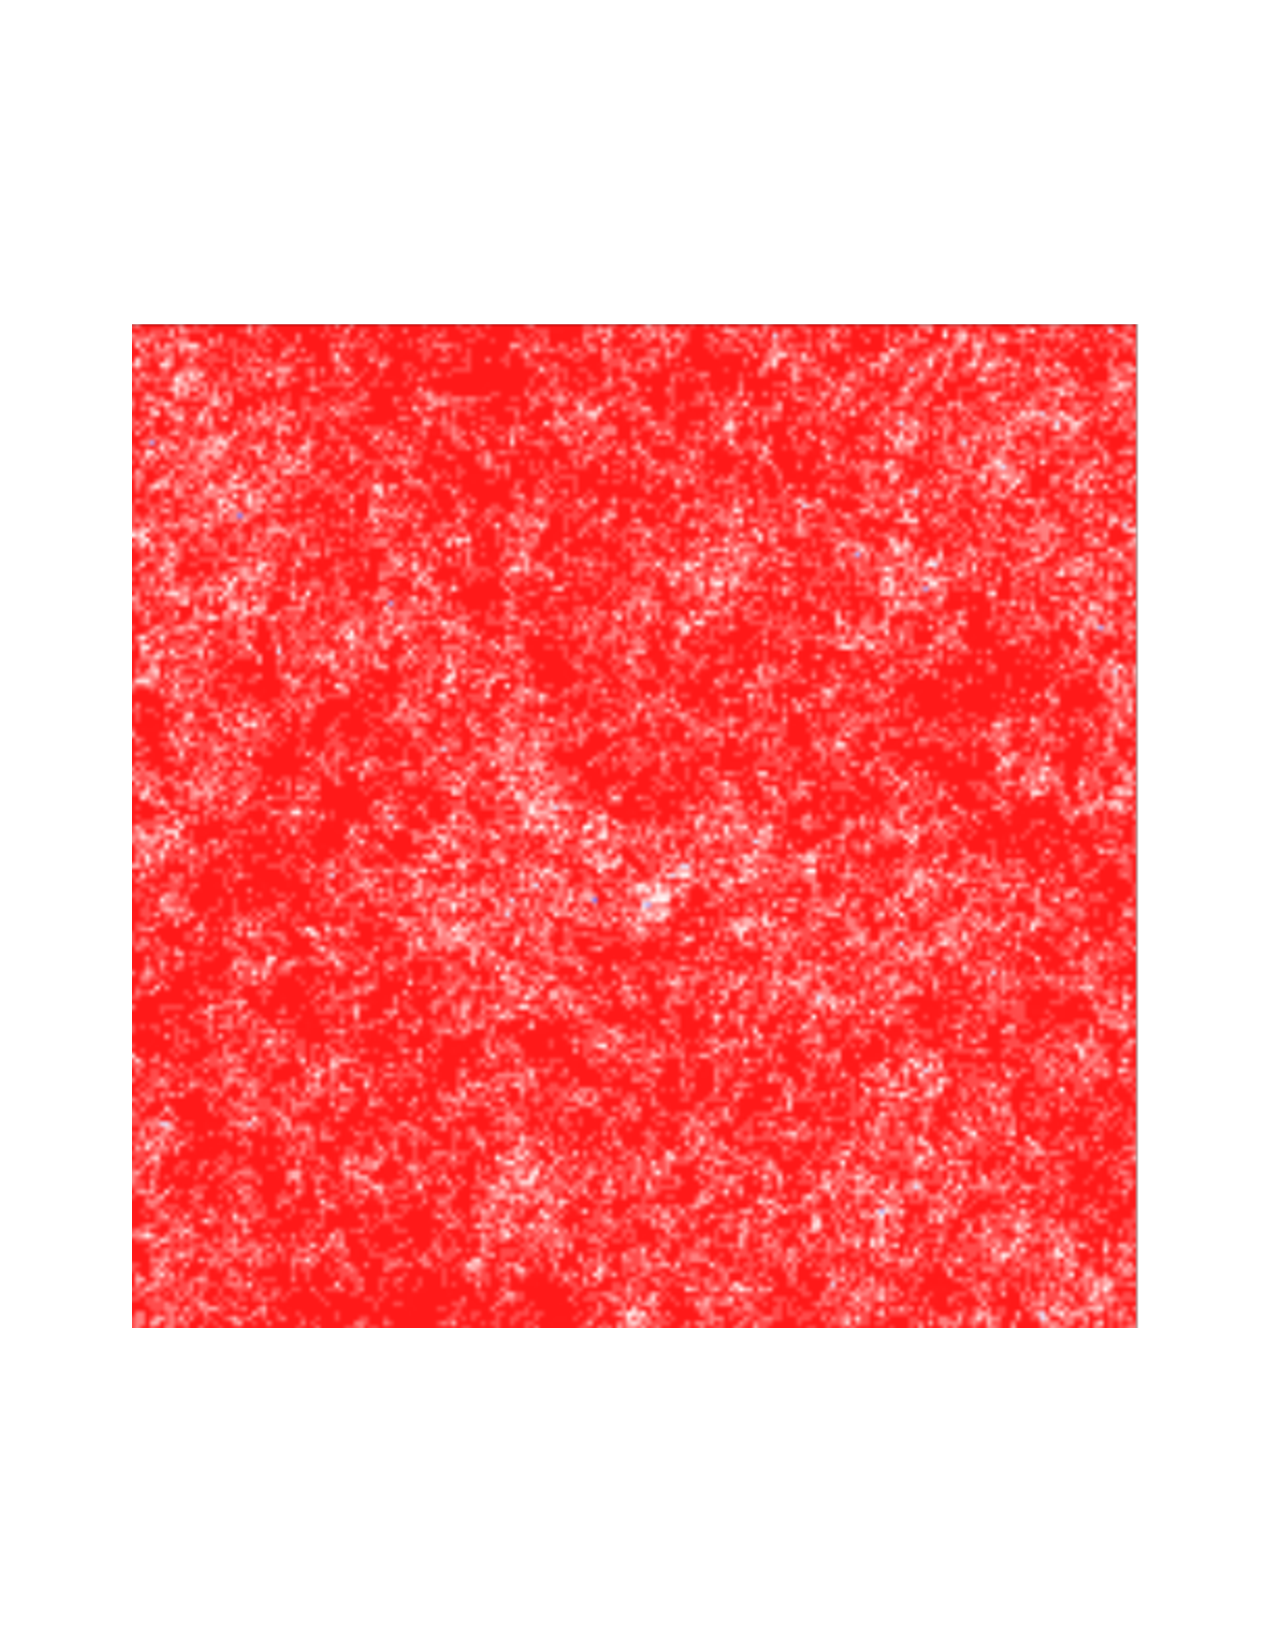
\includegraphics[width=7cm]{fus450_8_den.pdf} }}
    \caption {\small Density maps of FUS proteins obtained using the data from ARBD simulation}
    \label{fig:density}
\end{figure}
 
\begin{figure}[!ht]
    \centering
    \subfloat[Normalized density flunctuations of FUS at varying temperatures]{{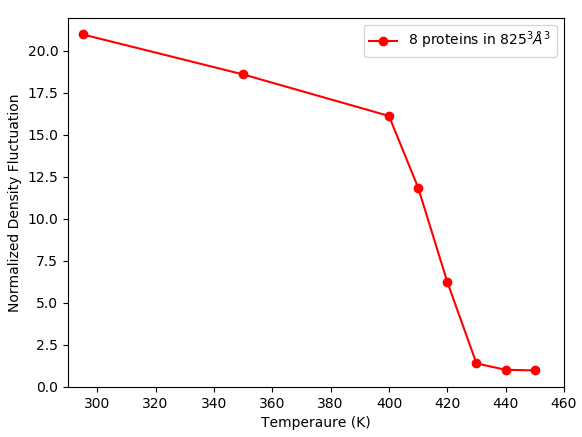
\includegraphics[width=7cm]{transition.png} }}
    \qquad
    \subfloat[FFT of the density maps of the trajectory data obtained from 8 ARBD simulations at 8 different temperatures of FUS simulated with the same conditions]{{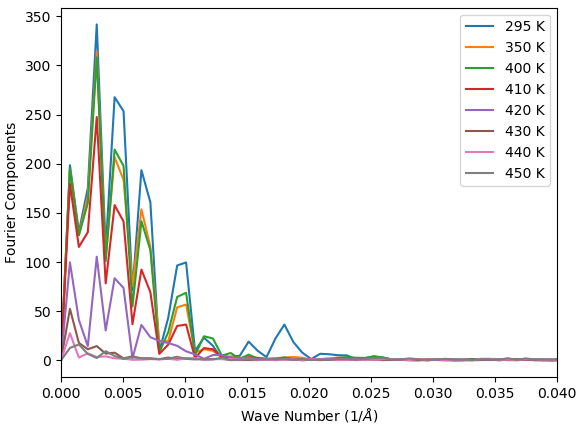
\includegraphics[width=7cm]{fft.png} }}
    \caption {\small Transition graph and FFT of the density of the FUS proteins at varying temperatures. 8 FUS proteins were run at various temperatures in 825$\mathring{A}^{3}$ resulting in 23.65 $\mu M$. The total number of atoms present were 43444. }
    \label{fig:fft}
\end{figure}

\begin{figure}[!ht]
    \centering
    \subfloat[Data obtained from all-atom MD trajectory of a single FUS protein in ionized water. Count is the number of contacts between tyrosine and arginine residues in the FUS protein.]{{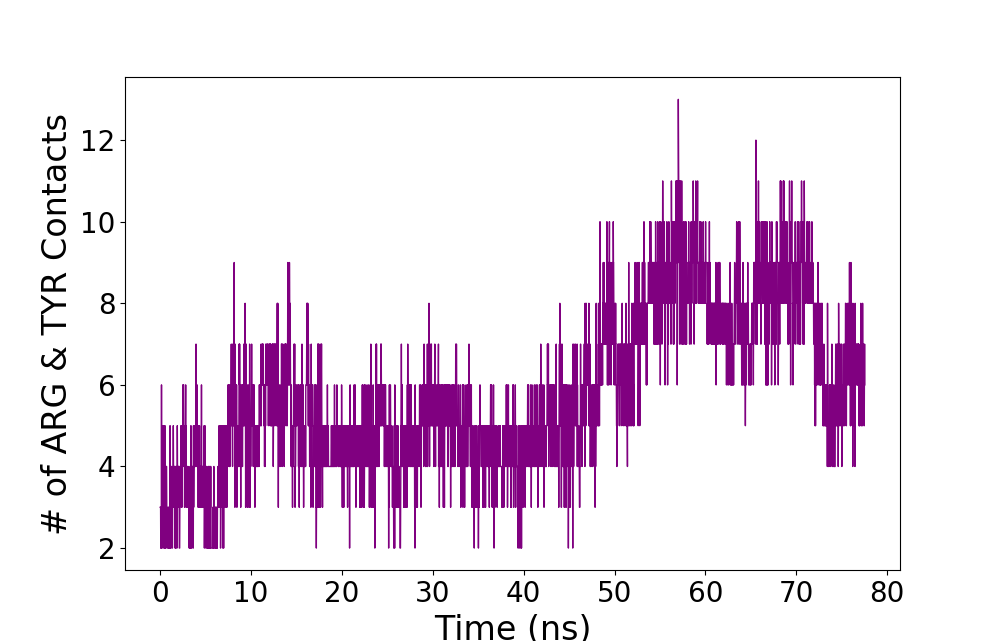
\includegraphics[width=8cm]{contacts.png} }}
    \qquad
    \subfloat[Representation of FUS protein, generated using VMD. Tyrosine and arginine residues are highlighted using blue and magenta, respectively.]{{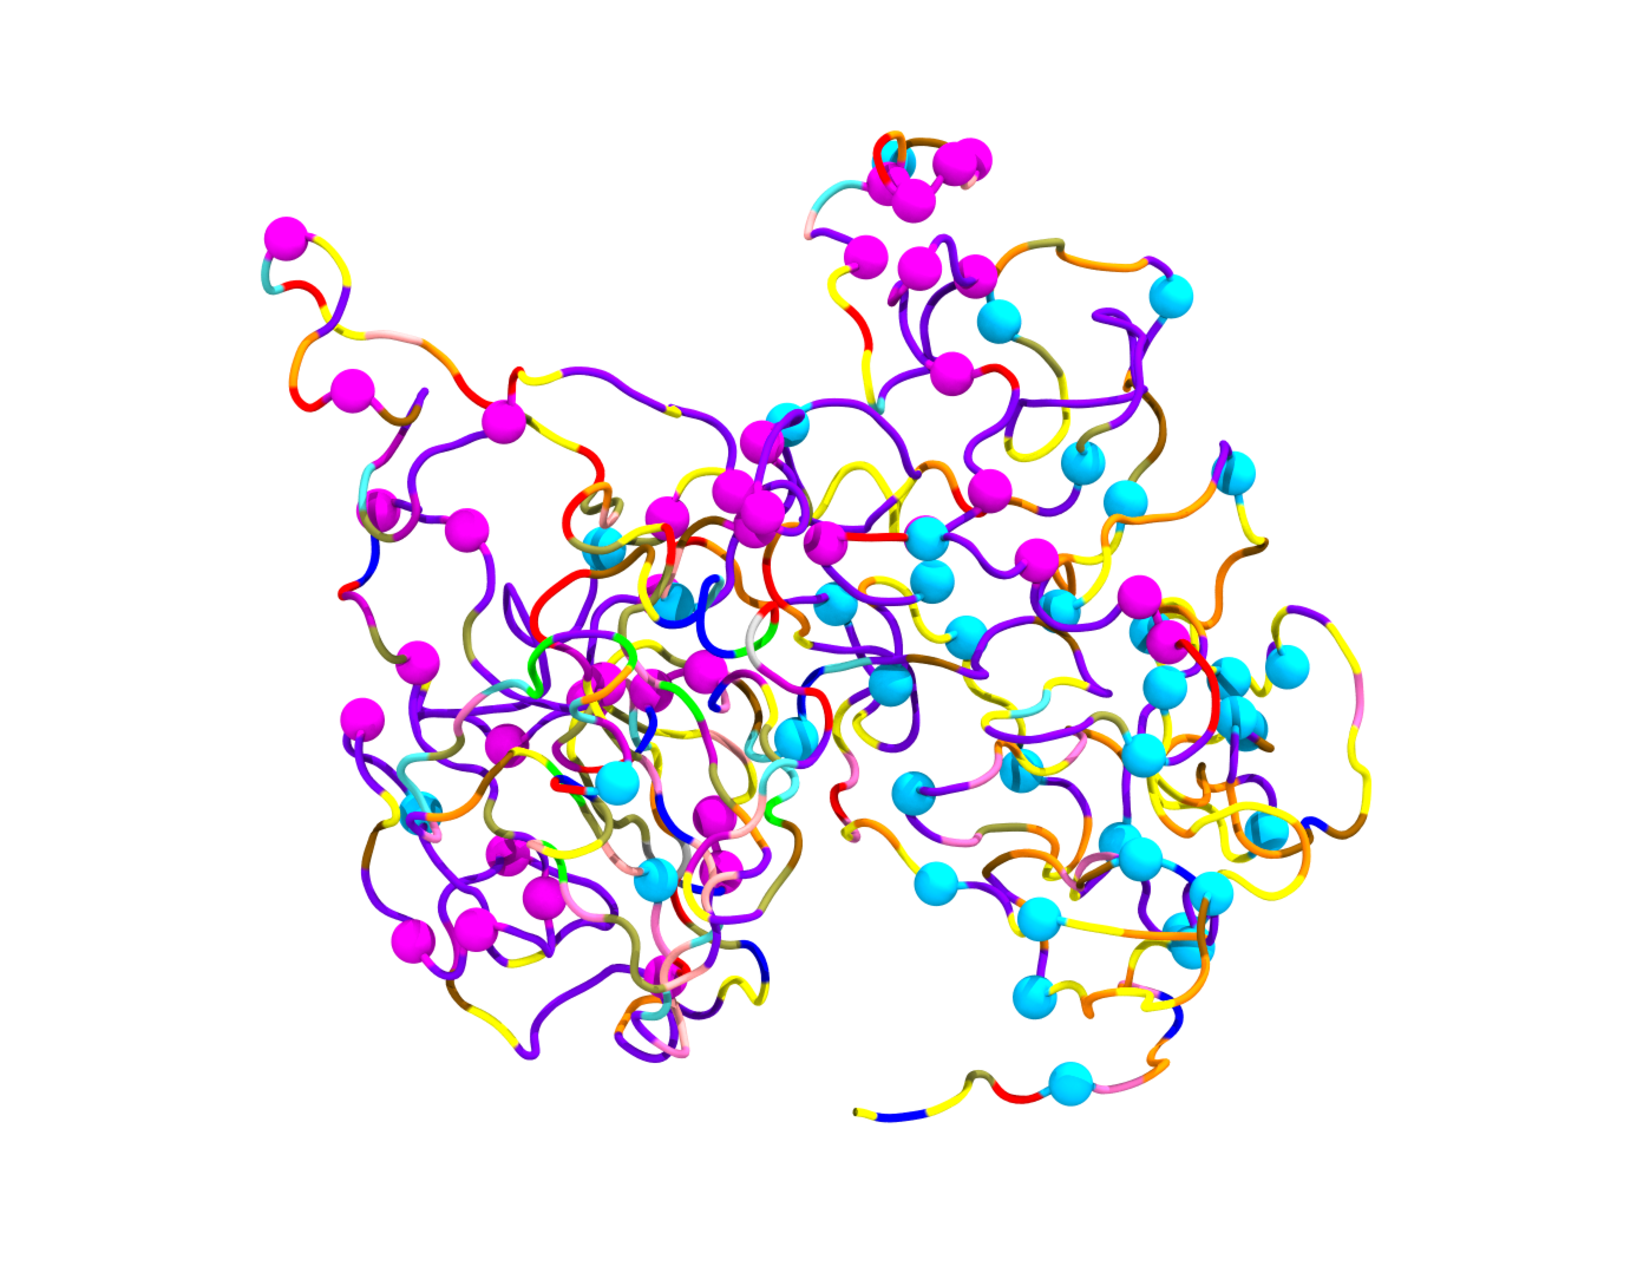
\includegraphics[width=6cm]{all_atom_arg_tyr6.pdf} }}
    \caption {\small Investigations of tyrosine and arginine residues in single FUS protein. }
    \label{fig:arg_tyr}
\end{figure}




\newpage

\section{Discussion}
The results of proteins undergoing liquid-liquid phase separation resembles liquid droplets, which is caused by the condensation into a dense phase \cite{Alberti_19}. LLPS is driven by the exchange of macromolecule/ 
water interactions for macromolecule/macromolecule and water/water interactions under conditions for which this process is energetically favorable \cite{Alberti_19}. Therefore, the LLPS process is sensitive to environmental conditions such as temperature and concentration also plays an important role. \\[0.01cm]

To investigate the temperature dependence of the LLPS process of FUS, 8 simulations are run for 10 $\mu s$. The state of the system at the end of 10 $\mu s$ ARBD simulation ran at $350$K appears to be clustered Fig.\ref{fig:fus_350}(b). In contrast, the system which was run at $450$K, Fig.\ref{fig:fus_430}(b), we can see that the proteins have not coalesced at all. By creating density maps of these, Fig.\ref{fig:density}, we can see that the distribution of the density map supports the results seen in Fig.\ref{fig:fus_350}(b) and \ref{fig:fus_430}(b). For the system that didn't coalesce Fig.\ref{fig:density}(b), the distribution of the density is more uniform unlike the other system, where we see a big dense region in the density map Fig.\ref{fig:density}(a) reflecting the cluster in \ref{fig:fus_350}(b).

Among the 10 simulations run at aforementioned temperatures for the 23.65 $\mu M$ system, around $415$K, we can see a transition from inhomogeneous to homogeneous phase n Fig.\ref{fig:fft}(a). We can clearly see that the normalized density fluctuations decreases as temperature increases indicating that for temperatures above $420$K, the density of the system remained almost the same as before. We can also observe an abrupt drop in normalized density fluctuations around $415$K. \\[0.01cm]

Fig.\ref{fig:fft}(b) shows the FFT of the density map against the wavenumber for systems at varying temperatures. If the system is inhomogeneous, there are more density fluctuations yielding closely spaced wave lengths and hence, a large wavenumber. On the other hand, if the system is homogeneous, the density fluctuations are more uniform resulting in larger wave lengths and hence, a small wavenumber. If the system is inhomogeneous, we would more peaks at larger wavenumbers as well as see peaks of larger magnitude. For a homogenous system, we would see very few peaks, if any at small wavenumber. We see an example of a homogenous system at $440$K, indicating that a condensate has not formed. Comparing the plot for $440$K and the plot for $295$K, we see many more peaks at $295$K indicating an inhomogeneous phase as phase separation occurs.  From Fig.\ref{fig:fft}(b), we see less homogeneity in the $295$K based on a smaller section of the data being at the zero line. \\[0.01cm]

From previous studies \cite{Wang_18}, we know that interactions between tyrosine and arginine residues are the principal drivers of LLPS, so one of the analysis includes counting the total number of contacts between the tyrosine and arginine residues over the $80 ns$ simulation, Fig.\ref{fig:arg_tyr}(a). \\[0.01cm]

Each simulation in this study took approximately 24 hrs to run when 1 unit of GPU is used for 23.65$\mu M$ system. To understand how concentration affects the phase separation process, higher concentration systems are being simulated at the same temperatures. However, these simulations take almost 3 times longer than the 23.65 $\mu M$ system so getting the results requires more time. The all-atom simulations take even longer than ARBD - they take about a week to simulate 100 $ns$. It is likely that there maybe ways to optimize the system to gain better computational run time. Given the duration of the internship and the availability of GPUs, we are limited in how many simulations we can run. Moreover, the process of writing code to analyze the MD and ARBD trajectories adds even more time. Even usage of supercomputers still have time constraints as there is a limit on how many node hours one job submission will have access per day. \\[0.01cm]
  
\newpage
\section{Conclusion}
Preliminary studies on interactions between tyrosine and arginine residues within a FUS protein were conducted using all-atom MD. The liquid-liquid phase separation process was studied using coarse-grained ARBD simulations. The liquid-liquid phase separation process is highly temperature dependent as at temperatures higher than $420$K, the proteins didn't coalesce at all. However, at room temperature or temperatures lower than $420$K, the proteins aggregate. Hence, the threshold temperature at which LLPS occurs appears to be at $420$K (see Fig.\ref{fig:fft}(a)). The VMD representations of the process as well as the analysis of the ARBD results previously presented all support this conclusion. All simulations conducted in this paper were done using the WT FUS protein. 

\section{Future Directions}
Additional simulations at various concentrations of FUS protein should be run to find out the concentration threshold for the LLPS process, akin to how we determined the temperature threshold in this paper. Another promising direction is to compare the relevant behavior of the WT FUS protein with that of the mutant FUS protein, which requires that we run analogous mutant FUS proteins simulations. The results of this comparison would provide insight into how certain mutations affect the phase separation properties of FUS. Moreover, it would help us determine exactly which regions of the protein are most involved in LLPS, for mutations in an essential region should disrupt the LLPS process much more than mutations in nonessential regions. 


\newpage


\bibliography{ref_ncsa}
\bibliographystyle{plain}
%[1] A. Patel, et al. A Liquid-to-Solid Phase Transition of the ALS Protein FUS Accelerated by Disease Mutation. Cell. 2015. [done]
%[2] A. Mullard, Biomolecular Condensates Pique Drug Discovery curiosity. Nature Reviews Drug Discovery 18, 324-326, 2019 [done]
%[3] S. Banani, Biomolecular Condensates: organizers of cellular biochemistry. Nature Reviews Molecular Cell Biology, 18:285, 2017 [done]
%[4] H. Deng, The role of FUS gene variants in neurodegenerative diseases. Nature Reviews Neurology volume 10, pages 337–348 (2014) [done]
%[5] J. Mittal, Sequence determinants of protein phase behavior from a coarse-grained model. PLOS Computational Biology. [2018] [done]
%[6] J. Wang, et al. A molecular grammar governing the driving forces for phase separation of prion-like RNA binding proteins. Cell. 2018. [done]
%[7] D. T. Murray, et al. Structure of FUS protein fibrils and its relevance to self-assembly and phase separation of low-complexity domains. Cell, 171:615–627, 2017 [done]

\end{document}